\documentclass[letterpaper, 12pt]{article}

%%%%%%%%%%%%%%%%%%%%%%%%%%%%%
% DEFINITIONS
% Change those informations
% If you need umlauts you have to escape them, e.g. for an ü you have to write \"u
\gdef\mytitle{\"Ubungsprotokoll}
\gdef\mythema{TDD with Groovy}

\gdef\mysubject{Softwareentwicklung}
\gdef\mycourse{4CHIT 2016/17}
\gdef\myauthor{Martin W\"olfer}

\gdef\myversion{0.2}
\gdef\mybegin{Begonnen am 1.3.2017}
\gdef\myfinish{Beendet am 4.3.2017}

\gdef\mygrade{}
\gdef\myteacher{}
%
%%%%%%%%%%%%%%%%%%%%%%%%%%%%%

%!TEX root=../document.tex

\usepackage[in]{fullpage}
% Fontencoding for possible copy&paste out of PDF
\usepackage[T1]{fontenc}
\usepackage[utf8]{inputenc}
\usepackage[ngerman]{babel}
\usepackage{graphicx} 
\usepackage{wasysym}
\usepackage{textcomp}
\usepackage{sectsty}
\usepackage{caption}
\usepackage{listings}
\usepackage{array}
\usepackage{nonfloat}
\usepackage{colortbl}
\usepackage{footmisc}
\usepackage{fancyhdr}
\usepackage{ccicons}
\usepackage{suffix}
\usepackage{multirow}
\usepackage{tabularx}
\usepackage{listings}
\usepackage{accsupp}
\usepackage{color}
\usepackage{url}
\usepackage[dvipsnames]{xcolor}
\usepackage[longnamesfirst,nonamebreak]{natbib}
\usepackage[headsep=1cm,headheight=3cm,hmargin=2cm,vmargin=2.5cm]{geometry}
\usepackage[nolist]{acronym}

% Definitions for Textcolor
\usepackage{color}
\definecolor{listings}{rgb}{0.96, 0.96, 0.96}
\definecolor{update}{rgb}{1, 0.8, 0.8}
\definecolor{config}{rgb}{0.8, 1, 0.8}
\definecolor{gray}{rgb}{0.4,0.4,0.4}
\definecolor{darkblue}{rgb}{0.0,0.0,0.6}
\definecolor{cyan}{rgb}{0.0,0.6,0.6}

% Java Syntaxhighligthning
% strings
\definecolor{javared}{rgb}{0.6,0,0}
% comments
\definecolor{javagreen}{rgb}{0.25,0.5,0.35}
% keywords
\definecolor{javapurple}{rgb}{0.5,0,0.35}
% javadoc
\definecolor{javadocblue}{rgb}{0.25,0.35,0.75}

\lstset{
	basicstyle=\ttfamily\small,
	keywordstyle=\bfseries\color[rgb]{0.496,0.000,0.332},
	commentstyle=\color[rgb]{0.246,0.496,0.371},
	stringstyle=\color[rgb]{0.164,0.000,0.996},
	tabsize=4,
	breaklines=true,
	numbers=left,
	numberstyle=\tiny\color{black},
	stepnumber=2,
	numbersep=8pt,
	numberstyle=\tiny,
	captionpos=b,
	xleftmargin=1cm,
	showspaces=false,
	showstringspaces=false,
	basewidth={0.53em,0.45em},
	frame=single,
	xleftmargin=1cm,
	basicstyle=\scriptsize,
}


\lstdefinestyle{Java}{
	language=Java,
	keywordstyle=\color{javapurple}\bfseries,
	stringstyle=\color{javared},
	commentstyle=\color{javagreen},
	morecomment=[s][\color{javadocblue}]{/**}{*/},
}

\lstdefinelanguage{XML}
{
	morestring=[b]",
	morestring=[s]{>}{<},
	morecomment=[s]{<?}{?>},
	stringstyle=\color{black},
	identifierstyle=\color{darkblue},
	keywordstyle=\color{cyan},
	% list your attributes here
	morekeywords={xmlns,version,type}
}

\lstdefinestyle{XML}{
	language=XML,
	basicstyle=\ttfamily\small,
	columns=fullflexible,
	commentstyle=\color{gray}\upshape
}

\newcommand{\noncopynumber}[1]{
	\BeginAccSupp{method=escape,ActualText={}}
	#1
	\EndAccSupp{}
}
\lstdefinestyle{bash}{
	language=bash,
	basicstyle=\ttfamily\small,
	literate={-}{{-}}{1},
	% http://tex.stackexchange.com/questions/145416/how-to-have-straight-single-quotes-in-lstlistings
	upquote=true;
	showstringspaces=false,
	%numbers=none,
	% http://tex.stackexchange.com/questions/122256/only-select-code-without-line-numbers
	numberstyle=\tiny\noncopynumber,
	breaklines=false,
	columns=fullflexible,
	basicstyle=\scriptsize
}

% http://tex.stackexchange.com/questions/83085/how-to-improve-listings-display-of-json-files
\colorlet{punct}{red!60!black}
\definecolor{background}{HTML}{EEEEEE}
\definecolor{delim}{RGB}{20,105,176}
\colorlet{numb}{magenta!60!black}
\lstdefinelanguage{json}{
	basicstyle=\ttfamily\small,
	numbers=left,
	numberstyle=\scriptsize,
	stepnumber=2,
	numbersep=8pt,
	showstringspaces=false,
	breaklines=true,
	literate=
	*{0}{{{\color{numb}0}}}{1}
	{1}{{{\color{numb}1}}}{1}
	{2}{{{\color{numb}2}}}{1}
	{3}{{{\color{numb}3}}}{1}
	{4}{{{\color{numb}4}}}{1}
	{5}{{{\color{numb}5}}}{1}
	{6}{{{\color{numb}6}}}{1}
	{7}{{{\color{numb}7}}}{1}
	{8}{{{\color{numb}8}}}{1}
	{9}{{{\color{numb}9}}}{1}
	{:}{{{\color{punct}{:}}}}{1}
	{,}{{{\color{punct}{,}}}}{1}
	{\{}{{{\color{delim}{\{}}}}{1}
	{\}}{{{\color{delim}{\}}}}}{1}
	{[}{{{\color{delim}{[}}}}{1}
	{]}{{{\color{delim}{]}}}}{1},
	basicstyle=\scriptsize
}

\usepackage[
	colorlinks,
	citecolor=black,
	filecolor=black,
	linkcolor=black,
	urlcolor=black,
	linktoc=all
]{hyperref}


\let\tempsection\section
\renewcommand\section[1]{\vspace{-0.3cm}\tempsection{#1}\vspace{-0.3cm}}
\WithSuffix\newcommand\section*[1]{\tempsection*{#1}}

\let\tempsubsection\subsection
\renewcommand\subsection[1]{\vspace{0cm}\tempsubsection{#1}\vspace{0cm}}

\let\tempsubsubsection\subsubsection
\renewcommand\subsubsection[1]{\vspace{0cm}\tempsubsubsection{#1}\vspace{0cm}}

\linespread{0.94}

\lhead{\mysubject}
\chead{}
\rhead{\bfseries\mythema}
\lfoot{\mycourse}
\cfoot{\thepage}
% Creative Commons license BY
% http://creativecommons.org/licenses/?lang=de
\rfoot{\ccby\hspace{2mm}\myauthor}
\renewcommand{\headrulewidth}{0.4pt}
\renewcommand{\footrulewidth}{0.4pt}

\begin{document}
\parindent 0pt
\parskip 6pt

\pagenumbering{Roman} 
%!TEX root=../laborprotokoll.tex

\begin{titlepage}

	\begin{figure}[!h]
		\begin{flushright}
			
\includegraphics[width=0.3\linewidth]{images/jdIT_tgm.png}
		\end{flushright}
	\end{figure}

	\vspace{2.5cm} 

	{\begin{center} \bfseries\huge
			\rule{17.5cm}{0.1mm}  
			\\[5mm]
			\mytitle\\[5mm]
			\mythema\\
			\rule{17.5cm}{0.1mm}  
	\end{center}}

	{\begin{flushright} \bfseries\Large
			\vspace{2cm}
			\mysubject\\
			\mycourse\\[10mm]
			\myauthor\\[10mm]
	\end{flushright}}

	{\begin{table}[!h] \bfseries\normalsize
		\begin{tabularx}{\textwidth}{lXr @{\hspace{0mm}}}
			&& Version \myversion\\
			\mygrade && \mybegin\\
			\myteacher && \myfinish\\
		\end{tabularx}
	\end{table}}

\end{titlepage}


\clearpage
\thispagestyle{empty}
\tableofcontents

\newpage
\pagenumbering{arabic}
\pagestyle{fancy}

%\vspace{-0.5cm}

%!TEX root=../document.tex

\section{Aufgabenstellung}
\begin{itemize}
	\item relevanter sourcecode
	\item Screenshot(s)
	\item Beispiel für mögliche sql injection, die durch Prepared Statements verhindert wird.
\end{itemize}

%!TEX root=../document.tex

\section{Testreports}
\subsection{Zusammenfassung}
\begin{minipage}{\linewidth}
	\centering
	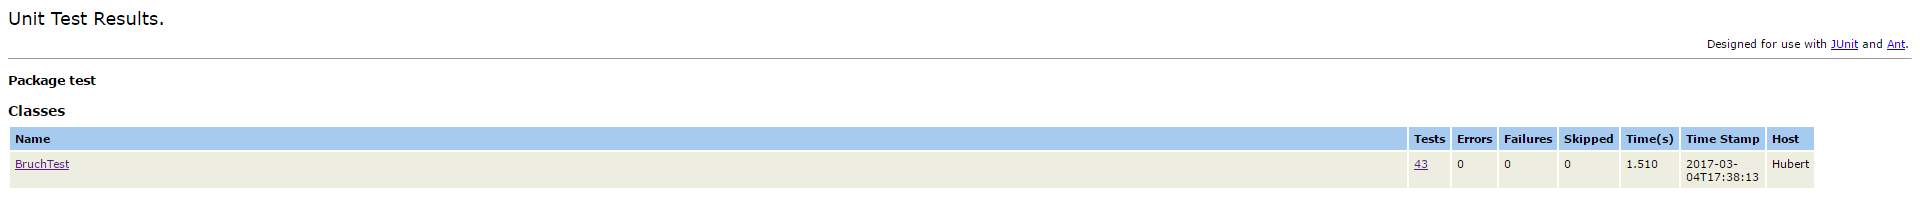
\includegraphics[width=1\linewidth]{images/pic1}
	\figcaption{Alle Tests wurden erfolgreich abgeschlossen}
\end{minipage}

\subsection{Einzelne Tests}
\begin{minipage}{\linewidth}
	\centering
	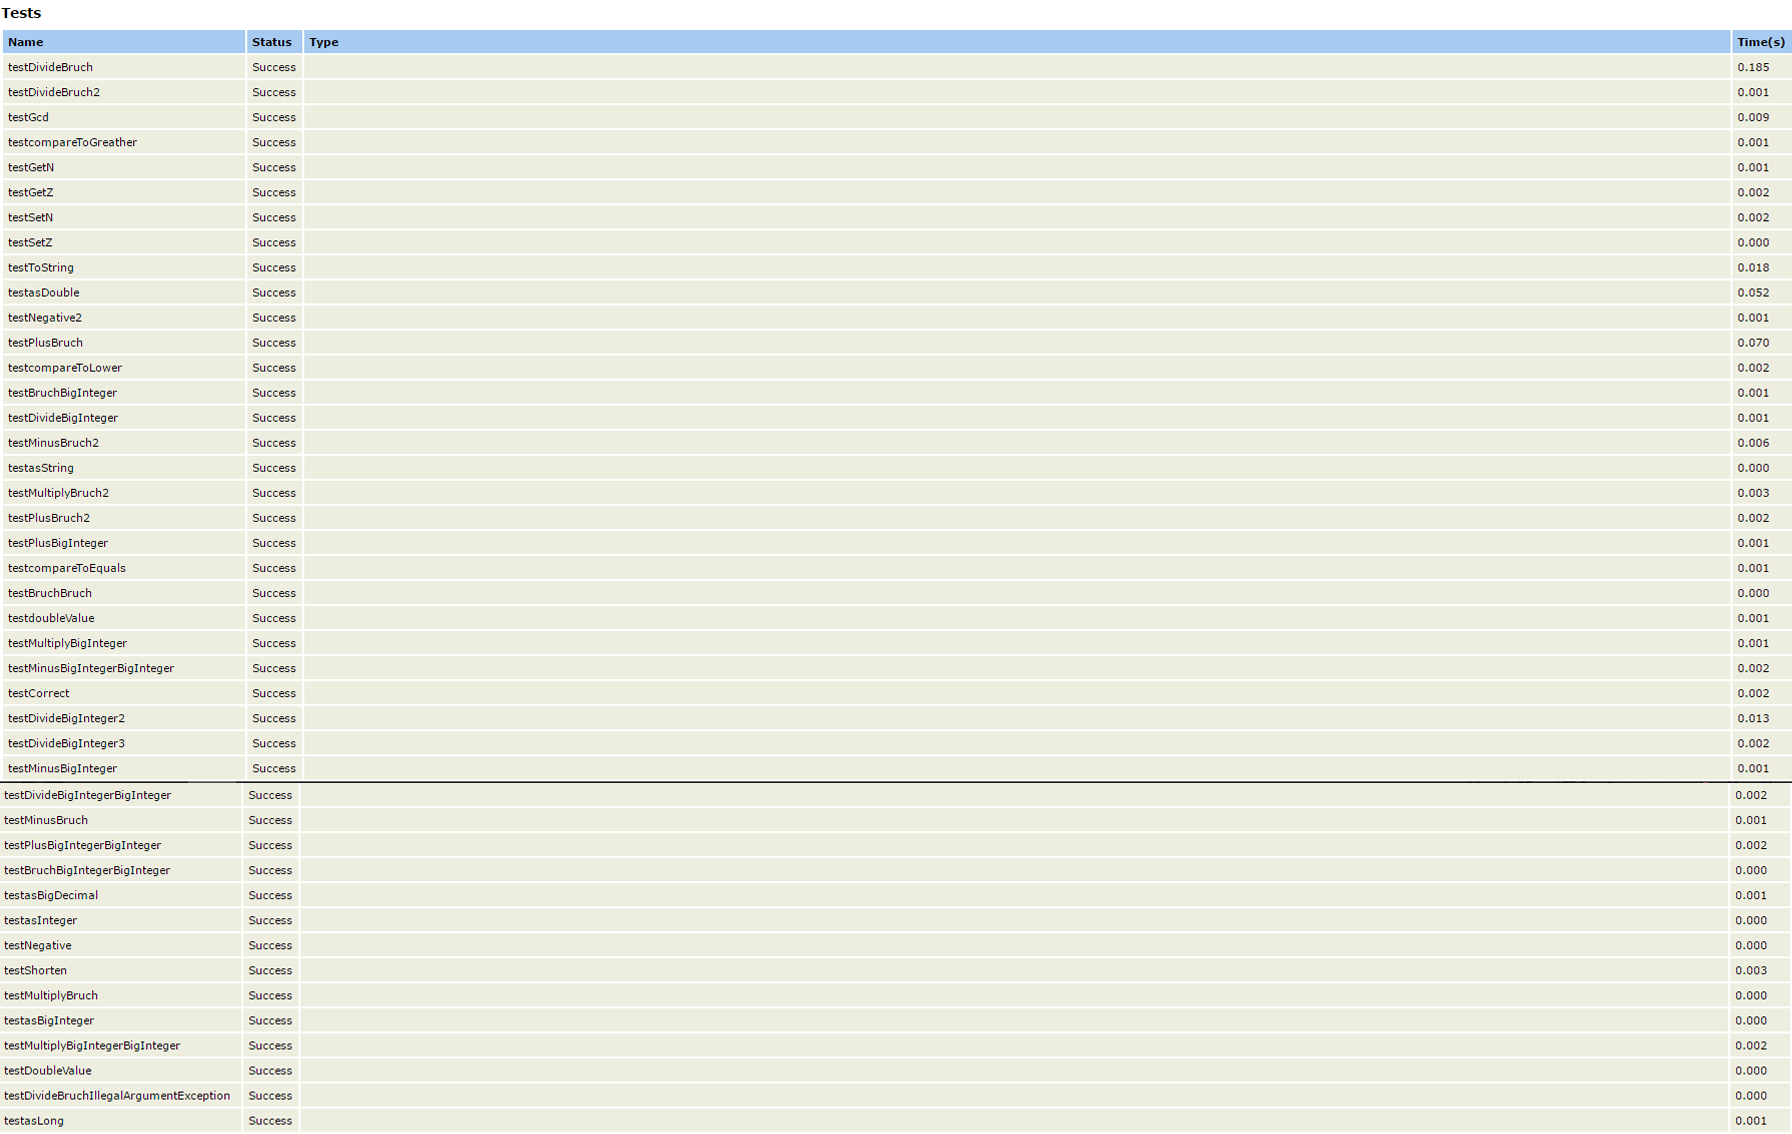
\includegraphics[width=1\linewidth]{images/pic4}
	\figcaption{Einzelne Tests wurden auch erfolgreich abgeschlossen}
\end{minipage}

\section{Coverage}
\begin{minipage}{\linewidth}
	\centering
	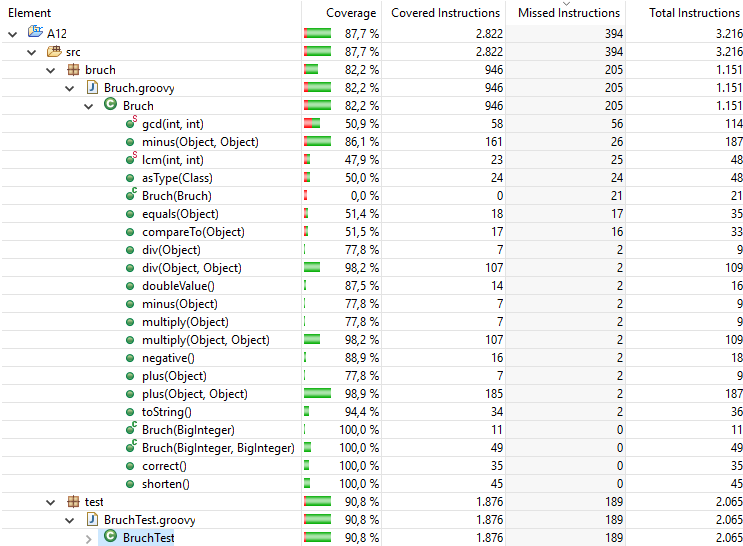
\includegraphics[width=1\linewidth]{images/pic5}
	\figcaption{Code-Coverage}
\end{minipage}

\section{Github}
\url{https://github.com/mwoelfer-tgm/java/tree/master/A12}

\clearpage

\end{document}
